\section{Results}
\label{sec:results}

\begin{figure}[pos=tbp]
\begin{center}
\includegraphics[width=0.47\textwidth]{img/results_clear-tiff-rgb.pdf}~
\includegraphics[width=0.47\textwidth]{img/results_clear-jpg-rgb.pdf}
%\vspace{-3mm}
\caption[resultsmodels]{Model results of predicting the 81 sample point locations for each of the four holdout test skies listed in \autoref{tab:testskies}. The final regression models are extra-trees (ETR), random-forest (RFR), k-nearest-neighbor (KNR) and linear (LNR). ETR performed the best, with a total error of 4-7.5\% RMSD across all 81 sample points. As expected, LNR was by far the worst performing. Note the similar results of using JPG captures versus minimally-processed, near raw TIFFs.}
\label{fig:results_models}
\end{center}
\end{figure}

\begin{figure}[pos=tbp]
\begin{center}
\begin{overpic}[width=0.46\textwidth]{img/05271015_measured.pdf}
\put(170,660){(a)}%
\end{overpic}%
~%
\begin{overpic}[width=0.46\textwidth]{img/05271015_predicted.pdf}
\put(170,660){(b)}%
\end{overpic}%
\\\vspace{2mm}%
\begin{overpic}[width=0.46\textwidth]{img/05271015_std.pdf}
\put(170,660){(c)}%
\end{overpic}%
~%
\begin{overpic}[width=0.46\textwidth]{img/05271015_ratio.pdf}
\put(170,660){(d)}%
\end{overpic}%
%\vspace{-1mm}
\caption[results05271015]{Whole sky results for holdout sky {05/27/2013 10:15} with ETR model. No ground truth sky samples from this capture were used for training. (a) and (b) show the 81 measured and predicted spectral radiance distributions; (c) shows the standard deviation from mean for both measured and predicted distributions; and (d) is the overall ratio between the two. Note the error in the ratio is within the absorption band near 1350 nm, where radiance is extremely small.}
\label{fig:results_05271015}
\end{center}
\end{figure}

Three of the four final regression models (ETR, RFR, KNR) resulted in very high R\textsuperscript{2} scores and acceptably low RMSD error on all holdout test skies listed in \autoref{tab:testskies}. As expected, the baseline LNR model resulted in relatively poor predictions across all test skies, with an overall error of 14-24\% RMSD. By contrast, ETR resulted in 4-7.5\% RMSD. For test sky 07/26/2013 13:15, three of the four models predicted within 4\% RMSD. In general, the tree-based models (ETR and RFR) perform better than the nearest-neighbor model (KNN). RMSD results for all models on each test sky are shown in \autoref{fig:results_models}. As mentioned in section \autoref{sec:method}, the sample azimuth feature affected results by 1-2\% RMSD, but otherwise scored as unimportant, and in fact its effect is within the standard deviation of error. We believe the sample azimuth feature could be safely dropped as a feature.

\autoref{fig:results_05271015} shows a comparison of all 81 measured and ETR predicted radiance distributions, their standard deviations, and overall averaged ratio between measured and predicted on test sky 05/27/2013 10:15. The difference in standard deviations of measured and predicted is minimal, and the averaged ratio is near $1.0$ for the majority of the spectrum (350-1780 nm). Note the erratic error in the ratio graph resides within an H$_{\text{2}}$O and CO$_{\text{2}}$ absorption band, where atmospheric radiance is extremely small \citep{lacis_absorption}, and measurements are susceptible to noise.

\begin{figure}[pos=tbp]
%\\\vspace{10mm}%
\begin{center}
\begin{overpic}[width=0.25\textwidth]{img/05271015.jpg}%
\put(135,755){\linethickness{0.25mm}\color{black}\line(-1,0){1000}}%11
\put(135,755){\color{black}\circle*{25}}%
\put(500,250){\linethickness{0.25mm}\color{black}\line(-2,-1){1000}}%56
\put(500,250){\color{black}\circle*{25}}%
\put(775,650){\linethickness{0.25mm}\color{black}\line(1,0){800}}%39
\put(775,650){\color{black}\circle*{25}}%
\put(570,570){\linethickness{0.25mm}\color{black}\line(2,-3){1000}}%74
\put(570,570){\color{black}\circle*{25}}%
\put(-1500,0){\includegraphics[width=0.36\textwidth]{img/05271015_s11.pdf}}%
\put(-1500,-1300){\includegraphics[width=0.36\textwidth]{img/05271015_s56.pdf}}%
\put(1100,0){\includegraphics[width=0.36\textwidth]{img/05271015_s39.pdf}}%
\put(1100,-1300){\includegraphics[width=0.36\textwidth]{img/05271015_s74.pdf}}%
\put(-1250,850){(11)}%
\put(-1250,-400){(56)}%
\put(1350,850){(39)}%
\put(1350,-425){(74)}%
\put(0,900){(a)}%
\end{overpic}%
\\\vspace{10mm}%
\begin{overpic}[width=0.25\textwidth]{img/05271015_wholesky.pdf}%
\put(925,0){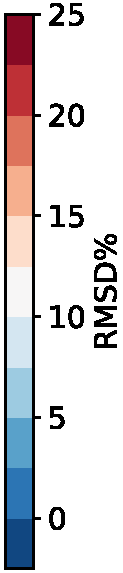
\includegraphics[width=0.0525\textwidth]{img/05271015_wholesky_cb.pdf}}%
\multiput(775,650)(0,80){14}{\line(0,1){40}}
\multiput(570,570)(0,80){14}{\line(0,1){40}}
\put(0,900){(b)}%
\end{overpic}%
\vspace{3mm}
\caption[wholesky05271015]{ETR results of four radiance predictions on holdout test sky 05/27/2013 10:15. (a) shows the camera processed JPG sky capture for convenience (the model was trained on TIFF data). (b) shows RMSD error across the entire sky. Radiance for samples (11), (56), (39) and (74) are pinpointed at their location in the sky. Samples (39) and (74) were the two worst predictions, with RMSD errors of 23.63\% and 21\% respectively.}
\label{fig:wholesky_05271015}
\end{center}
\end{figure}

For the same holdout test sky (05/27/2013 10:15), \autoref{fig:wholesky_05271015} shows ETR prediction error across the entire hemispherical sky, and highlights the two worst spectral radiance predictions (23.63\% and 21\% RMSD). These two measurements occur near the sun's corona, where radiance values are traditionally higher and more erratic than the rest of a clear sky. Two other predictions selected at random are shown for comparison. A vast majority of the 81 samples are predicted to within 1\% RMSD. Note that even with ``high'' error, predicted curves align with ground truth measurements in terms of shape. The models therefore have learned the wavelength relative intensities of the sky in accordance with capture time, sun location, etc. This is consistent with nearly all predicted results; while the magnitudes per wavelength sometimes deviate, the general shapes each predicted curve is accurate.

Although we were expecting some insight from providing multiple exposures of sky images, results seem to indicate that HDR data, at least for clear skies, does not improve model prediction. All HDR runs resulted in very similar error to non-HDR runs. Similarly, differences in results between 0.25 s, 1 s, and 2 s exposures were also insignificant. We believe this may be because clear sky color changes are so ``uniform'' throughout the day, that multiple exposures lack significance. In other words, all provided exposures may have had the same color change trends. We suspect that HDR data will be more significant in the reconstruction of spectral radiance for scattered and overcast skies, as the color variations of clouds are less uniform across exposures.

\begin{figure}[pos=tbp]
\begin{center}
\begin{overpic}[width=0.48\textwidth]{img/results_color_07261315.pdf}
\put(150,610){(a)}%
\end{overpic}%
~%
\begin{overpic}[width=0.48\textwidth]{img/results_color_09241539.pdf}
\put(150,610){(b)}%
\end{overpic}%
\vspace{-1mm}
\caption[resultscolor]{Sky color model made little to no difference in training and prediction results. (a) and (b) show RMSD results on 07/26/2013 13:15 and 09/24/2013 13:15 respectively.}
\label{fig:results_color}
\end{center}
\end{figure}

Results of our color experiment (\autoref{fig:results_color}) seem to indicate that color model is irrelevant to our method. This implies that our method can be used with any representation of color, as the trends in color across the sky are similar regardless of format. It is unclear if using color data initially captured in an sRGB format somehow restricted the range of the other color models after conversion. In other words, would initially capturing the sky in a color model that maps to a larger color space be better?

\begin{figure}[pos=tbp]
\begin{center}
\includegraphics[width=0.55\textwidth]{img/results_resolution.pdf}
\vspace{-2mm}
\caption[resultsresolution]{Limiting resolution to 5 nm drastically decreases model size, improves computation speed, and even increases prediction success, likely because the prediction problem becomes simpler with $^1$/$_5$ the number of radiance values to predict. Further reductions yield diminishing returns.}
\label{fig:results_resolution}
\end{center}
\end{figure}

The results of the spectral resolution experiment (\autoref{fig:results_resolution}) show the benefits of decreasing spectral resolution from 1 to 5 nm. Model sizes (particularly the large ensemble models), as well as model training and prediction times, decrease significantly. The improvements in prediction accuracy are likely due to the radiance curve being more smooth, i.e. fewer peaks and valleys for the regression model to learn, as well as a simpler prediction problem in general, i.e. fewer outputs to predict. The size of the training dataset also decreases with reduced resolution, but that is eclipsed by the largest model sizes. Beyond 5 nm resolution, further reductions result in diminishing returns. This is an important find for real-time applications, which may operate on limited embedded hardware.

We note here that results between the minimally processed, uncompressed TIFF sky images and traditional, camera processed, compressed JPG sky images, were roughly the same (\autoref{fig:results_models}). TIFF data resulted in only slightly better results ($\mathtt{\sim}$1\%) on some skies, though that may be within the standard deviation of prediction error and machine learning random fluctuation. In terms of storage space and processing, the TIFF images ($\mathtt{\sim}$35 MB) are roughly 15 times larger than the JPG images compressed with quality level 100 ($\mathtt{\sim}$2.5 MB). Given the similar results, we recommend the use of JPG captures for real-time applications of our method.

\begin{figure}[pos=tbp]
\begin{center}
\begin{overpic}[width=0.6\textwidth]{img/sradmaps.jpg}%
\put(-55,600){(a)}%
\put(-55,370){(b)}%
\put(-55,120){(c)}%
\put(100,755){(1)}%
\put(350,755){(2)}%
\put(590,755){(3)}%
\put(840,755){(4)}%
\end{overpic}%
%\vspace{-2mm}
\caption[resultssradmapall]{Columns (1-4) are the holdout test skies in \autoref{tab:testskies}, in respective order. Rows (a) and (b) show traditional, camera processed JPG and minimally processed TIFF captures, respectively. Row (c) shows the sradmap visualizations generated for skies in row (b); we use our ETR model to predict spectral radiance (350-1780 nm) for every pixel of test sky image, sum the radiance distribution, and visualize with a false-color map.}
\label{fig:results_sradmapall}
\end{center}
\end{figure}

\begin{figure}[pos=tbp]
\begin{center}
\includegraphics[width=0.25\textwidth]{img/07261315_sradmap_gray.png}%
\hspace{2mm}%
\includegraphics[width=0.25\textwidth]{img/07261315_sradmap.png}%
\hspace{2mm}%
\includegraphics[width=0.1\textwidth]{img/sradmap_cbs.jpg}%
%\vspace{-1mm}
\caption[resultssradmap0726]{False-colored sradmap visualizations for holdout test sky 07/26/2013 13:15. Each pixel plotted is a summation of an entire spectral radiance distribution (350-1780 nm). There is no significance to the summation algorithm; it is simply used to visualize the data.}
\label{fig:results_sradmap_0726}
\end{center}
\end{figure}

Spectral radiance files (sradmaps) are the culminating whole sky output of our methods. They are generated by extracting features per pixel of test skies (\autoref{tab:testskies}) and feeding them through any one of our models. Linear scale false-color visualizations of ETR model predicted sradmaps are shown in \autoref{fig:results_sradmapall} and \autoref{fig:results_sradmap_0726}. Test sky images were first scaled down to a resolution of 333x333 pixels, to anticipate real-time processing speeds. sradmap generation, visualization, and logged output took $\mathtt{\sim}$20 s to complete on the same machine specified in \autoref{ssec:resolution}; embedded hardware would likely take longer. Visualization of sradmap and logged output are not necessary for real-time applications.